% Template LaTeX document for CSSR4Africa Deliverables
% Adapted from documents prepared by EPFL for the RobotCub project
% and subsequently by the University of Skövde for the DREAM project
%
% DV 28/06/2023

\documentclass{CSSRforAfrica}

\usepackage[hidelinks,colorlinks=false]{hyperref}
\usepackage[titletoc,title]{appendix}
\usepackage{latexsym}
% \usepackage[a4paper, margin=1in]{geometry} % Adjust margins as needed
\usepackage{pdflscape}

\usepackage[table]{xcolor} % For row colors
\usepackage{longtable}      % For tables that span multiple pages
%\usepackage{geometry}       % Optional: Adjust page margins
%\usepackage{lmodern}        % Optional: Enhanced font
\usepackage{fontenc}        % Optional: Better font encoding
\usepackage{caption}        % Optional: Customize captions
\usepackage{longtable}
\usepackage{dirtree}
\usepackage{listings}
\usepackage{array}
\usepackage{float}

\usepackage{tikz}
\usetikzlibrary{positioning}
\usepackage{graphicx}

%%% for listing ; added by Pam %%%%%%%%%%%%%%%%%%%%%%%%%%%%%%
\captionsetup[figure]{format=hang}
\definecolor{codegreen}{rgb}{0,0.6,0}
\definecolor{greenyellow}{rgb}{0.8, 0.7, 0.10}
\definecolor{backcolour}{rgb}{0.95,0.95,0.95} 

\definecolor{codepurple}{rgb}{0.58,0,0.82}
\definecolor{codered}{rgb}{0.65,0,0}
\definecolor{codeblue}{rgb}{0,0,0.8}

\lstdefinestyle{withoutNumbering}{
    backgroundcolor=\color{backcolour},  
    commentstyle=\color{codegreen},
    keywordstyle=\color{magenta},
    stringstyle=\color{purple},
    basicstyle=\small\fontfamily{DejaVuSansMono-TLF}\selectfont,
    breakatwhitespace=false,        
    breaklines=true,                
    captionpos=b,                    
    keepspaces=true,                
    showspaces=false,                
    showstringspaces=false,
    showtabs=false,                  
    tabsize=2,
}

\lstdefinestyle{log}{
    backgroundcolor=\color{backcolour},  
    commentstyle=\color{codegreen},
    keywordstyle=\color{magenta},
    stringstyle=\color{purple},
    basicstyle=\ttfamily\footnotesize, ,
    breakatwhitespace=false,        
    breaklines=true,                
    captionpos=b,                    
    keepspaces=true,                
    showspaces=false,                
    showstringspaces=false,
    showtabs=false,                  
    tabsize=2,
    % literate{=}{{\textequals}}1
}

\usepackage{listings}
%\usepackage{xcolor} # not necessary. why was it causing a problem? REMEMBER to Check


% Custom C++ style
\lstdefinestyle{cppstyle}{
    backgroundcolor=\color{backcolour},   
    commentstyle=\color{codegreen},
    keywordstyle=\color{codered}\bfseries,
    stringstyle=\color{codepurple},
    basicstyle=\small\fontfamily{DejaVuSansMono-TLF}\selectfont,             
    showspaces=false,                
    showstringspaces=false,
    showtabs=false,                  
    tabsize=2,
    language=C++,
    morekeywords={nullptr, constexpr, override, final, noexcept, alignof, alignas, 
                 decltype, char16_t, char32_t, concept, requires, BT},
    emph={std, string, vector, map, set, unordered_map, unordered_set,
         pair, shared_ptr, unique_ptr, array, tuple, optional, variant, KeyValueType, CultureKnowledgeBase},
    emphstyle=\color{codeblue},
    morecomment=[s]{/*}{*/},
    morecomment=[l]//,
    morestring=[b]",
    escapeinside={(*@}{@*)},
}

\newcommand{\blank}{~\\}
\newcommand{\checkbox}{{~~~~~~~\leavevmode \put(-7,-1.5){  \huge $\Box$  }}}

\begin{document}
\input{epsf}

%%
%% SHOULD NOT NEED TO BE CHANGED BEFORE THIS POINT
%% ------------------------------------------------
%%

\deliverable{D5.4.3}                   % REPLACE with correct number
\title{D5.4.3 Robot Mission Interpreter}    % REPLACE with correct title

\leadpartner{Carnegie Mellon University Africa}  
\partner{The University of the Witwatersrand}       

\revision{1.8}                         
\deliverabledate{31/12/2024}   
\submissiondate{16/12/2024}  
\revisiondate{07/06/2025}      
\disseminationlevel{PU}
\responsible{Tsegazeab Tefferi, CMU-Africa}         


%%
%% Create the titlepage
%%

\maketitle
 
 
\section*{Executive Summary}
%==================

\label{executive_summary}
%%\addcontentsline{toc}{section}{Executive Summary}
 
Deliverable D5.4.3 focuses on the development of the \texttt{\small Robot Mission Interpreter} module, a central component within the CSSR4Africa software architecture. This module, also referred to as \texttt{\small behaviorController} ROS node, serves as the orchestrator for interpreting and executing robot mission specifications defined in Task 5.4.2, effectively bridging high-level mission planning with low-level robot execution. By leveraging the BehaviorTree.CPP library, the \texttt{\small behaviorController} node interprets XML-based mission scripts.

The \texttt{\small Robot Mission Interpreter} integrates seamlessly with eight distinct ROS nodes, including \texttt{\small animateBehavior}, \texttt{\small overtAttention}, \texttt{\small gestureExecution}, \texttt{\small textToSpeech}, \\ \texttt{\small robotNavigation}, \texttt{\small tabletEvent}, \texttt{\small speechEvent}, and \texttt{\small robotLocalization}. These interactions are facilitated through ROS service calls and publish-subscribe mechanisms, allowing the module to control behaviors such as animating lifelike patterns, executing gestures, navigating environments, processing speech inputs, and detecting human presence. This comprehensive integration ensures that the robot can effectively engage with its environment and perform mission-critical tasks.

The development process encompasses a structured software engineering methodology, including requirements definition, module design, coded implementation, and unit testing, all adhering to the standards outlined in Deliverable D3.2 Use Case Scenario Definition.

In the work plan, this deliverable is assigned to the University of the Witswatersrand. However, the material in this version was developed and written by Carnegnie Mellon University Africa. This was necessary because the Wits version was not available and, without it, it is not possible to build a complete, operational system and demonstrate the required CSSR4Africa functionality. 
\newpage
 
 
%\graphicspath{{./figs/}}
\pagebreak
~\vspace{-19mm} % to avoid an orphan on the next page
\tableofcontents
\newpage



\section{Introduction}
%=============

This document describes the development and implementation of a ROS node for the execution of robot missions on the Pepper robot. The Robot Mission Interpreter functions as a central ROS node within the CSSR4Africa software architecture, orchestrating system behavior through ROS service calls and publish-subscribe mechanisms. It performs two key functions translating  Robot Mission Specifications into executable robot commands, and processing real-time sensor data and status updates from other ROS nodes to guide robot behavior.



\begin{figure}[htbp]
    \centering
    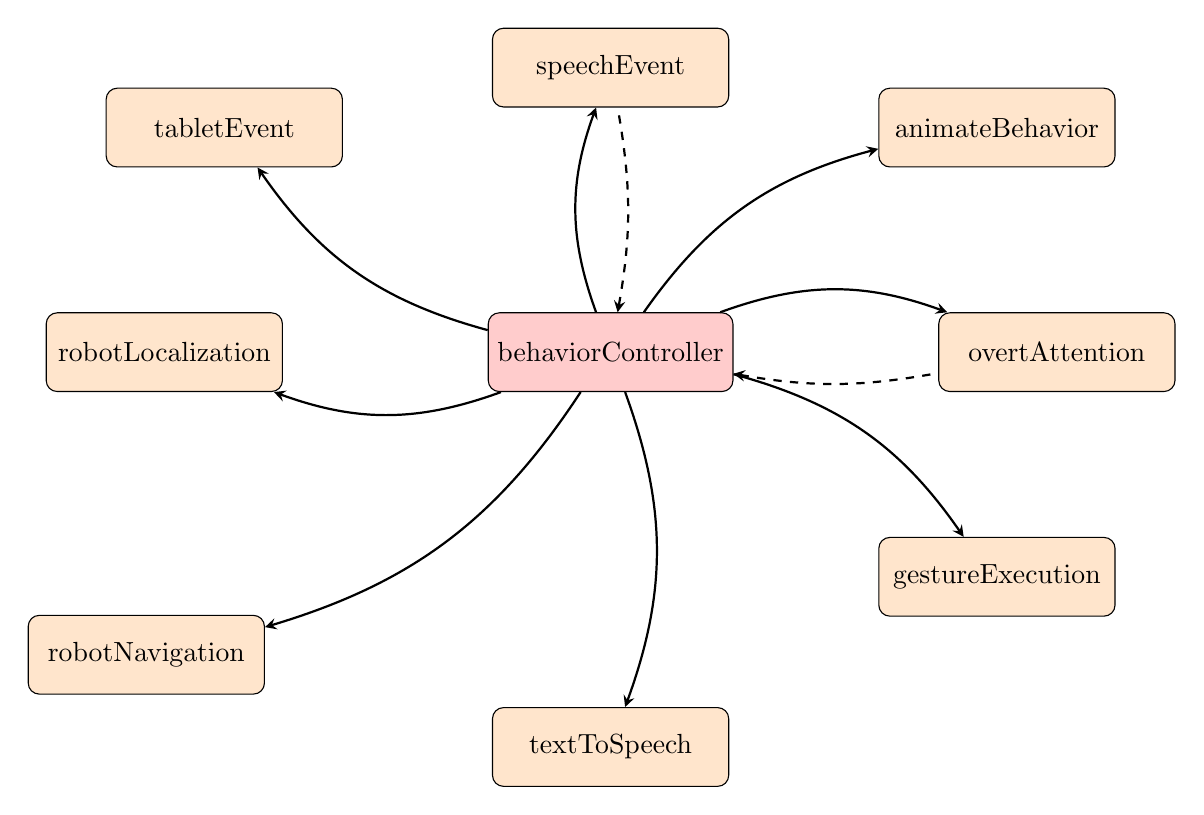
\begin{tikzpicture}[
        node distance=2.6cm,
        every node/.style={draw, rectangle, rounded corners, minimum width=3cm, minimum height=1cm, align=center},
        central/.style={fill=red!20},
        peripheral/.style={fill=orange!20},
        arrow/.style={->, thick, >=stealth},
        reverse/.style={<-, thick, >=stealth, dashed}
    ]
        % Central Node
        \node[central] (interpreter) {behaviorController};
        
        % Peripheral Nodes
        \node[peripheral, above right=of interpreter] (animateBehavior) {animateBehavior};
        \node[peripheral, right=of interpreter] (overtAttention) {overtAttention};
        \node[peripheral, below right=of interpreter] (gestureExecution) {gestureExecution};
        \node[peripheral, below=4cm of interpreter] (textToSpeech) {textToSpeech};
        \node[peripheral, left=of interpreter] (robotLocalization) {robotLocalization};
        \node[peripheral, above left=of interpreter] (tabletEvent) {tabletEvent};
        \node[peripheral, above=of interpreter] (speechEvent) {speechEvent};
        \node[peripheral, below left=4cm of interpreter] (robotNavigation) {robotNavigation};
        
        % Arrows with slight bend to avoid overlap
        \foreach \node in {animateBehavior, overtAttention, gestureExecution, textToSpeech, 
                          robotNavigation, tabletEvent,robotLocalization, speechEvent} {
            \draw[arrow] (interpreter) to[bend left=20] (\node);
        }

            \foreach \node in {overtAttention, speechEvent} {
    
    \draw[reverse] (interpreter) to[bend right=10] (\node);
    }
        
    \end{tikzpicture}
    \caption{Interaction Diagram of the Robot Mission Interpreter Node with other ROS Nodes}
    \label{fig:interaction_diagram}
\end{figure}

Figure~\ref{fig:interaction_diagram} illustrates the communication architecture of the Robot Mission Interpreter. The central node, shown in red, coordinates with eight peripheral ROS nodes shown in orange. The bidirectional communication is represented by arrows: solid arrows indicate service call from the interpreter to the nodes, while dashed arrows topic messages sent from the nodes to the interpreter.


This deliverable presents a comprehensive report detailing each phase of the software development lifecycle for the Robot Mission Interpreter module. Section 2 outlines the requirements definition process, aligning functional necessities with the project's overarching goals, thereby establishing the foundation for subsequent development efforts.

Section 3 delves into the module design, documenting the module's dependencies including the \texttt{\small BehaviorTree.CPP} library and the knowledge bases which contain cultural and environmental knowledge utilized during mission executions. The subsection explaining the mission execution framework provides detailed insights into critical components such as the \texttt{\small initializeTree} function (3.2.1), the Blackboard mechanism (3.2.2), custom Action and Condition Nodes (3.2.3), and the \texttt{\small HandleFallback} Action Node (3.2.4). The interface design is addressed with a focus on data exchange mechanisms utilizing ROS middleware and file input/output operations.

Section 4 describes the implementation of the module, including file organization and the configuration of various essential files. This includes external dependencies (4.1.1), main source files (4.1.2), configuration files (4.1.3), robot mission specifications (4.1.4), service definition files (4.1.5), message definition files (4.1.6), and package relevant files (4.1.7). Further details on the configuration file (4.2), input file (4.3), output file (4.4), topics file (4.5), topics subscribed (4.6), topics published (4.7), services supported (4.8), services called (4.9), and robot mission nodes (4.10) are provided to ensure a clear understanding of the module's operational setup.

Section 5 focuses on executing missions, detailing the prerequisites (5.1), the execution process (5.2), and the procedures for switching missions (5.3). Finally, Section 6 outlines the unit testing strategies, covering test configuration (6.1) and the launching of tests (6.2), ensuring the reliability and accuracy of the module's functionalities.


\newpage
\section{Requirements Definition}
%====================

The \texttt{\small behaviorController} node is a vital component of the CSSR4Africa software system, responsible for interpreting robot mission specifications developed in Task 5.4.2 by implementing the use case scenarios outlined in \textnormal{Deliverable D2.1 User Case Scenario Definition}. This deliverable is essential for identifying and addressing specific user expectations, ensuring that the node can accurately interpret and execute diverse mission scenarios across various operational environments, including both the physical robot and the simulator.

At its core, the \texttt{\small behaviorController} must proficiently parse mission specifications from a file written in the custom script language defined in \textnormal{Deliverable D5.4.2 Robot Mission Language}, comprehending both syntax and semantics to extract meaningful instructions that dictate robot behaviors. It must orchestrate complex interaction dynamics between the robot and visitors, faithfully executing all defined behaviors and interaction protocols as specified in \textnormal{Deliverable D5.4.2 Robot Mission Language}.

The node must interact seamlessly with various CSSR4Africa modules to perform tasks and process relevant information. To achieve this, it must communicate with eight different nodes by subscribing to two topics and making service calls to six servers. These interactions enable functionalities such as animating behaviors, executing gestures, controlling navigation, managing overt attention mechanisms, and initiating and processing interactions with humans.

The module must operate in two distinct modes: normal and verbose. In normal mode, the module executes mission scenarios without additional logging. In contrast, verbose mode allows the module to provide detailed information by printing logs to the terminal, which is invaluable for debugging and monitoring purposes. Additionally, the module must function with Automatic Speech Recognition (ASR) either enabled or disabled. When ASR is enabled, the module must processes human speech to facilitate audio-based interactions. When disabled, interactions must be managed through touch or physical inputs via the robot’s tablet, allowing for alternative methods of communication.

Furthermore, the module must ensure robustness and reliability in mission execution by continuously monitoring the performance of nodes it communicates with and initiate fallback behaviors when necessary. It must employ  error detection and recovery mechanisms to gracefully handle errors, service call failures, and unexpected behaviors, thereby maintaining system stability.

% Lorem ipsum dolor sit amet, consectetur adipiscing elit, sed do eiusmod tempor incididunt ut labore et dolore magna aliqua.
%  \\~\\
% \

\newpage
\section{Module Design}
%==============

The Robot Mission Interpreter module serves as the central orchestrator of the CSSR4Africa software architecture. It processes robot mission specifications defined in Task 5.4.2, interpreting and executing each action and condition node within the specification. Operating as a mission coordinator, it combines XML-based mission specifications with real-time inputs from other nodes and relevant information from the Knowledge Base, executing custom internal logic for each action and condition node to generate appropriate control commands.

As the primary control node of the system, it acts as the coordination layer between high-level mission planning and low-level robot execution.
Operating within the ROS framework, this module interfaces with other nodes in the CSSR4Africa software package through ROS service calls and publish-subscribe mechanisms. 
It maintains active communication channels with eight different nodes, orchestrating their operations to achieve the specified mission objectives by executing various robot behaviors.
\begin{enumerate}
    \item \texttt{\small animateBehavior}: Triggers the execution of life-like behavioral patterns to foster human-robot interaction
    \item \texttt{\small gestureExecution}: Initiates specific body and hand gestures through the robot's motion control system
    \item \texttt{\small overtAttention}: Initiates the robot's attention system to focus on specific environmental features or locations relevant to social interaction
    \item \texttt{\small robotLocalization}: Determines the current pose of the robot.
    \item \texttt{\small robotNavigation}: Directs the robot's movement system to navigate to specified locations or follow predetermined paths
    \item \texttt{\small speechEvent}: Activates speech recognition processes to capture and process human verbal inputs
    \item \texttt{\small tabletEvent}: Triggers the display of contextually appropriate interaction menus on the robot's tablet interface
    \item \texttt{\small textToSpeech}: Commands the robot to deliver verbal messages through its speech synthesis system
\end{enumerate}

The \texttt{\small behaviorController} node operates in two distinct modes: normal and verbose. In normal mode, the module executes mission scenarios with minimal output. In verbose mode, it provides comprehensive logging information to the terminal, facilitating debugging and system monitoring. The module also supports two interaction modes based on Automatic Speech Recognition (ASR) configuration. With ASR enabled, the module can process verbal commands through speech recognition. With ASR disabled, the module relies on the robot's tablet interface for touch-based interactions and physical inputs. These operational modes are configured through the \texttt{\small behaviorControllerConfiguration.ini} file.


\subsection{Dependencies}
%- - - - - - - - - - - - - - - - - - - - - 

The \texttt{\small behaviorController} node has the following external dependencies that are essential for its core functionality. These dependencies provide fundamental capabilities required for proper operation of the module and must be properly configured during setup.

\subsubsection{BehaviorTree.CPP}
%- - - - - - - - - - - - - - - - - - - - - 

BehaviorTree.CPP is an open-source C++ library designed to implement, read, and execute behavior trees. It utilizes an external Domain-Specific Language (DSL) instead of an internal one, as internal DSLs can hinder the maintainability and analyzability of the behavior model in the long term \cite{Ghzouli2023}. The library employs template metaprogramming instead of code generation, which provides a degree of type safety when implementing custom tree nodes without requiring users to engage with specialized code-generation tools, making the library feel akin to using a regular C++ library \cite{Ghzouli2020}. 

Trees in BehaviorTree.CPP are defined using a Domain-Specific scripting language based on XML, allowing them to be loaded at run-time; this means that even if the trees are written in C++, their morphology is not hard-coded, offering greater flexibility \cite{BehaviorTreeWebsite}. They can be created using any text editor, but this library provides a user-friendly graphical editor called Groot \cite{Dortmans2022}. A more detailed description of how the robot mission specifications are developed is explained in \textnormal{D5.4.2 Robot Mission Language}.

BehaviorTree.CPP was one of only two libraries out of 18 surveyed to have ROS support, be open-source, have a GUI tool to design missions, and be written in C++ \cite{Iovino2020}. It is popular, with 3.1k stars on GitHub, and the repository remains actively maintained with continuous contributions and updates as of December 15, 2024 \cite{BehaviorTreeGithub}. It is currently being used in essential ROS2 packages, such as the Nav2 navigation stack \cite{ROSNavigation}. Version 4.0 of the software was released in October of 2022 and was presented at ROSCon 2022 in Japan \cite{ROSCon2022}.

The \texttt{\small behaviorController} node was built by importing the fundamental components from this library, including the core behavior tree types, the XML parsing functionality for loading tree specifications at runtime, and the tree execution engine. This dependency provides all the necessary building blocks for constructing and executing behavior trees while allowing the mission interpreter to focus on implementing the specific behaviors and actions.

\subsubsection{eSpeak}
%-------------------------------
eSpeak is a compact, open-source text-to-speech (TTS) synthesizer available for Linux, Windows, Android, and other platforms. Supporting over 100 languages and accents, it is designed to be lightweight while offering broad linguistic coverage.

While the resulting speech is clear and can be produced at high speeds, it is less natural or smooth compared to larger synthesizers based on human speech recordings.

The software is available as a command-line program (for both Linux and Windows), capable of speaking text from files or standard input (stdin).\cite{eSpeakWebsite}.

eSpeak is not strictly required for the normal operation of the \texttt{behaviorController} node, but it becomes useful during debugging, particularly when vocalizing the names of action and condition nodes being executed, along with their parameters.

\newpage
\subsubsection{Knowledge Base}
%- - - - - - - - - - - - - - - - - - - - - 

The Knowledge Base is a critical component of the CSSR4Africa software architecture, serving as a centralized data store containing essential information for the Pepper robot to operate effectively. It functions as the primary source of data upon which the \texttt{\small behaviorController} node depends, providing comprehensive details relevant to the robot's operational context.

Within this centralized repository, two main categories of knowledge are stored: \textnormal{Cultural knowledge information}, as detailed in \textnormal{D5.4.1 Cultural Knowledge Ontology \& Knowledge Base}, and \textnormal{Environmental knowledge information}, defined in \textnormal{D5.4.2 Robot Mission Language}. Cultural knowledge allows the Pepper robot to perform tasks in a culturally sensitive manner, ensuring respectful interactions within specific cultural contexts. Environmental knowledge equips the robot with critical physical information necessary for safe navigation and effective interaction with its surroundings.

The Knowledge Base is made available within the "Utilities" software package, which includes both cultural and environmental knowledge base files alongside the software components required for accessing and retrieving stored values. Its internal organization adheres to the directory structure outlined in \textnormal{D3.2 Software Engineering Standards Manual}. The contents merge code deliverables from \textnormal{D5.4.1} and \textnormal{D5.4.2} into a single, unified package to enhance ease of use, access, and maintainability.




\paragraph{Environment Knowledge}\mbox{}%\\ 
%- - - - - - - - - - - - - - - - - - - - - 

The Environment Knowledge Base is an organized repository explicitly developed to formally represent and store physical information about the robot's environment, facilitating robot navigation and interaction within its surroundings.

Utilizing the ontology defined in \textnormal{D5.4.2 Robot Mission Language}, the Environment Knowledge Base systematically stores environmental parameters as key-value pairs within the file ``environmentalKnowledgeBaseInput.dat," located in the ``data" directory of the ``Utilities" package. Each key-value pair comprises an alphanumeric key paired with numeric or alphanumeric values that encapsulate the environment knowledge.

Access to this environmental information is managed through the specialized C++ helper class named \texttt{\small EnvironmentalKnowledgeBase}, also defined in \textnormal{D5.4.2 Robot Mission Language}. This class serves as the primary interface to the knowledge base, efficiently managing file access and providing public methods for enabling retrieval of stored environmental parameters.

Specifically tailored for the \textnormal{``Lab Tour''} scenario described in \textnormal{D2.1 Use Case Scenario Definition}, the \texttt{\small EnvironmentalKnowledgeBase} helper class encapsulates the necessary functionality for retrieving exhibit information, the robot's home location, and other critical details required to guide the robot's behavior and decision-making processes during its missions.

Code snippets illustrating the data structures used to represent these specifications, methods for accessing the data, detailed examples demonstrating the use of the class to read the environment knowledge base file, and practical examples showing how to retrieve values associated with a robot location given its identification number and how to retrieve the sequence of robot locations involved in a tour are provided in \textnormal{D5.4.2 Robot Mission Language}.

\paragraph{Cultural Knowledge}\mbox{}\\
%- - - - - - - - - - - - - - - - - - - - - 

The Cultural Knowledge Base is a structured system explicitly developed to formally represent and store culturally sensitive knowledge, specifically tailored for African contexts, with a particular emphasis on Rwandan culture. The ontology defining this cultural knowledge was initially provided in document \textnormal{D1.2 Rwandan Cultural Knowledge}. Subsequently, based on this ontology, a repository was implemented as described in document \textnormal{D5.4.1 Cultural Knowledge Ontology \& Culture Knowledge Base}. This repository comprises cultural parameter values, enabling robots to exhibit culturally appropriate and respectful behaviors, activities, actions, and motions during interactions with Rwandan individuals.

Technically, the system organizes cultural knowledge into key-value pairs, stored within the file ``cultureKnowledgeBaseInput.dat", located in the ``data" directory of the ``Utilities" package. Each key-value pair consists of an alphanumeric key and an associated numeric or symbolic value, explicitly capturing aspects of cultural information.

Access to this structured cultural information is facilitated through a specialized C++ helper class named ``CultureKnowledgeBase", which serves as the primary interface to the knowledge base. This helper class efficiently manages file access and provides two public methods, notably the critical ``getValue()" function, enabling seamless retrieval of stored cultural parameters.

The \texttt{\small behaviorController} is the sole accessor to the Cultural Knowledge Base, serving as the central distributor of all cultural knowledge required by other nodes within the system, such as retrieving appropriate gesture parameters for respectful gestures for the \texttt{\small gestureExecution} ROS node and providing accurate distance values for culturally sensitive navigation to the \texttt{\small robotNavigation} ROS node.

One such example of cultural knowledge usage is the language used to conduct the current mission. This value is stored in the Cultural Knowledge Base's ``cultureKnowledgeBaseInput.dat" file under the key ``\texttt{\small PhraseLanguage}". During initialization, this value is retrieved using the ``\texttt{\small getValue()}" accessor method and then transmitted to the \texttt{\small speechEvent} ROS node. This transmission occurs once during initialization and subsequently each time a request is made to the \texttt{\small /textToSpeech/say\_text} service

\begin{lstlisting}[style=cppstyle]
   KeyValueType keyValue;
   CultureKnowledgeBase culturalKnowledgebase;

   culturalKnowledgebase.getValue("PhraseLanguage", &keyValue);
   std::string missionLanguage = keyValue.alphanumericValue;

   //make service call to /speechEvent/setLanguage
   //store in blackboard for use by /textToSpeech/say_text service

\end{lstlisting}

\newpage
\subsection{Mission Execution}
%--------------------------

The mission execution process is the core functionality of the \texttt{\small behaviorController} node. It involves the interpretation and execution of robot mission specifications defined in XML format, as described in \textnormal{D5.4.2 Robot Mission Language}, using the BehaviorTree.CPP library. This process begins by parsing the XML file that defines the mission specification, which includes hierarchical nodes. The library instantiates these nodes and initializes a ``BehaviorTree'' object. During execution, the root node is recursively ``ticked'', with control nodes orchestrating the execution of child nodes, while leaf nodes interface with tasks that make up the selected scenario, as described in \textnormal{D2.1 Use Case Scenario Definition}. Node statuses (``Success'', ``Failure'', ``Running'') propagate dynamically, enabling real-time adaptation to environmental feedback. A shared \textnormal{``Blackboard''} facilitates data exchange between nodes, ensuring parameterization and state persistence. This reactive loop allows the Pepper robot to adjust the mission on-the-fly.

Underpinning this process are several critical components, detailed below, each of which plays a crucial role in ensuring the successful execution of the mission.
\subsubsection{The \texttt{\small initializeTree} function}

The function \texttt{\small BT::Tree initializeTree(std::string missionSpecification)} is responsible for preparing the behavior tree for execution based on the robot mission specification given in XML format. It performs three critical steps:

\begin{enumerate}
    \item \textnormal{File Loading:} The function accepts a mission specification name as input and constructs the full file path by appending a ``.xml'' extension and locating it in the module's data directory. 

    \item \textnormal{Node Registration:} Before the tree can be created, all custom Action and Condition nodes that will be used in the mission must be registered with the behavior tree factory. This is accomplished using the template function:
    \begin{lstlisting}[style=cppstyle]
template <typename T, typename... ExtraArgs>
void registerNodeType(const std::string& ID, ExtraArgs... args)
    \end{lstlisting}
    This registration step is crucial - if the XML specification references a node type that hasn't been properly registered, the \texttt{\small behaviorController} will encounter a fatal error when the tree's execution reaches that node.

    \item \textnormal{Tree Creation:} Finally, the function uses BehaviorTree.CPP's factory method:
    \begin{lstlisting}[style=cppstyle]
BT::Tree BehaviorTreeFactory::createTreeFromFile(
    const std::filesystem::path& file_path)
    \end{lstlisting}
    to parse the XML specification and construct an executable behavior tree. This factory method handles the creation of all nodes, establishes their connections according to the XML structure, and returns a fully initialized \texttt{\small BT::Tree} object ready for execution.
\end{enumerate}

\subsubsection{Blackboard}
%- - - - - - - - - - - - - - - - - - - - - 

The Blackboard serves as a centralized key/value storage mechanism that facilitates data sharing across all nodes within a Behavior Tree \cite{BehaviorTreeWebsite}. It provides two essential functions in the module. 

First, it enables information sharing between different nodes executing within the same behavior tree. This is crucial for coordinating actions and maintaining state across different branches of the tree.

Second, since action and condition nodes have limited lifespans that end after their execution, the Blackboard acts as a persistent storage solution. Any data that needs to survive beyond a node's execution cycle must be stored in the Blackboard for future access.

An important point to note is that the Blackboard doesn't need to be explicitly created- it's automatically instantiated during tree initialization. Each action and condition node has access to it through the \texttt{\small config} object.



\subsubsection{Custom Action and Condition Nodes}
%- - - - - - - - - - - - - - - - - - - - - 

In a robot mission specification implemented using behavior trees, the composite nodes (Control Nodes and Decorator nodes) are provided by the BehaviorTree.CPP library. Custom implementations are necessary exclusively for Leaf Nodes, which consist of Action and Condition nodes.

\paragraph{Class Definition}\mbox{}\\
%- - - - - - - - - - - - - - - - - - - - - 

Each Leaf Node is implemented as a C++ class that inherits from either \texttt{\small BT::SyncActionNode} or \texttt{\small BT::ConditionNode}, depending on whether it represents an Action or a Condition node. The class definition includes the following components:

\subparagraph{1. Constructor}
%- - - - - - - - - - - - - - - - - - - - - 

The constructor for an Action node follows the 
\begin{lstlisting}[style=cppstyle]
    BT::SyncActionNode(const std::string& name, const NodeConfig& config)
\end{lstlisting}
%\texttt{\small BT::SyncActionNode(const std::string\& name, const NodeConfig\& config)} 
signature, while that for a Condition node follows the 
%\texttt{\small BT::ConditionNode(const std::string\& name, const NodeConfig\& config)}
\begin{lstlisting}[style=cppstyle]
    BT::ConditionNode(const std::string& name, const NodeConfig& config)
\end{lstlisting}
signature. During initialization, the constructor sets up necessary ROS components, such as service clients and topic subscribers, to facilitate the node's functionality.

\subparagraph{2. Tick Method}
%- - - - - - - - - - - - - - - - - - - - - 

\begin{lstlisting}[style=cppstyle]
    BT::NodeStatus tick()
\end{lstlisting}

The \texttt{\small tick()} method encapsulates the core logic of each Leaf Node and is invoked during behavior tree traversal. Serving as the primary execution method for both Action and Condition nodes, \texttt{\small tick()} performs the node's specific functionality, which may include modifying Blackboard values, making service calls to CSSR4Africa ROS nodes, or executing custom actions based on messages received from subscribed topics.

This method returns one of three possible states:
\begin{itemize}
    \item \texttt{\small BT::NodeStatus::SUCCESS}: Execution completed successfully.
    \item \texttt{\small BT::NodeStatus::FAILURE}: Execution failed.
    \item \texttt{\small BT::NodeStatus::RUNNING}: Execution is ongoing (applicable only to Action nodes).
\end{itemize}

\subparagraph{3. Private Section}
%- - - - - - - - - - - - - - - - - - - - - 

The private section contains:
\begin{itemize}
    \item Class member variables shared between the constructor and the \texttt{\small tick()} method.
    \item Callback methods for handling topic subscriptions.
    \item Other implementation-specific private members essential for the node's operation.
\end{itemize}

\subsubsection{\texttt{\small HandleFallBack} Action Node}
%- - - - - - - - - - - - - - - - - - - - - 

The \texttt{\small HandleFallback} action node is an important component within the \\ \texttt{\small behaviorController}, that must be able to manage error recovery mechanisms when preceding actions encounter failures. Although its logic is not yet implemented, the \texttt{\small HandleFallback} node is intended to provide robust fallback strategies to ensure mission continuity and system resilience. Upon activation, typically triggered by a failure in a prior action node, \texttt{\small HandleFallback} will assess the nature of the failure and determine the appropriate recovery approach. This can involve executing a default recovery procedure that attempts to restore the system to a safe or initial state or invoking a custom, action-specific recovery function tailored to address the specific failure context. 

Work is currently in progress to identify a suitable recovery strategy for the \\ \texttt{\small HandleFallback} node that can ensure that it can effectively manage a wide range of failure scenarios and maintain mission integrity under adverse conditions.

%\subsubsection{Data Specifications}
%- - - - - - - - - - - - - - - - - - - - - 

\newpage
\section{Implementation}
%=================

\subsection{File Organization}
%------------------------
The \texttt{\small behaviorController} node's codebase is organized into two primary components: the external dependency \texttt{\small BehaviorTree.CPP} and the core \texttt{\small behaviorController} module. 

The \texttt{\small behaviorController} module follows a standard ROS package structure with dedicated directories for configuration files, mission data, service definitions, message specifications, and build configurations.

\vspace*{0.5em}
\renewcommand*\DTstyle{\ttfamily}
{\footnotesize
\begin{figure}[htbp]
    \dirtree{%
        .1 cssr\_system.
        .2 BehaviorTree.CPP.
        .2 behaviorController.
        .3 CMakeLists.txt.
        .3 CSSR5AfricaLogo.svg.
        .3 README.md.
        .3 config.
        .4 behaviorControllerConfiguration.ini.
        .4 cultureKnowledgeBaseConfiguration.ini.
        .4 environmentKnowledgeBaseConfiguration.ini.
        .3 data.
        .4 cultureKnowledgeBaseInput.dat.
        .4 cultureKnowledgeValueTypesInput.dat.
        .4 environmentKnowledgeBaseInput.dat.
        .4 labTour.xml.
        .3 include.
        .4 behaviorController.
        .5 behaviorControllerInterface.h.
        .5 cultureKnowledgeBaseInterface.h.
        .5 environmentKnowledgeBaseInterface.h.
        .3 msg.
        .4 overtAttentionMode.msg.
        .3 src.
        .4 behaviorControllerApplication.cpp.
        .4 behaviorControllerImplementation.cpp.
        .4 cultureKnowledgeBaseImplementation.cpp.
        .4 environmentKnowledgeBaseImplementation.cpp.
        .3 srv.
        .4 animateBehaviorSetActivation.srv.
        .4 gestureExecutionPerformGesture.srv.
        .4 overtAttentionSetMode.srv.
        .4 robotLocalizationSetPose.srv.
        .4 robotNavigationSetGoal.srv.
        .4 speechEventSetLanguage.srv.
        .4 speechEventSetStatus.srv.
        .4 tabletEventPromptAndGetResponse.srv.
        .4 textToSpeechSayText.srv.
        }

    \caption{File structure of the Robot Mission Interpreter}
    \label{fig:main_node_file_structure}
\end{figure}
}
\newpage
\subsubsection{External Dependencies}
%- - - - - - - - - - - - - - - - - - - - - 
\begin{itemize}
    \item \texttt{\small BehaviorTree.CPP}: This directory houses the source code for the external \textnormal{BehaviorTree.CPP} library, an essential dependency for the \texttt{\small behaviorController} node. Including the library's source code directly alongside the module ensures seamless integration and distribution, allowing for the use of the module right from the get go without having to install the library separately.
\end{itemize}

\subsubsection{Main Source Files}
%- - - - - - - - - - - - - - - - - - - - - 
\begin{itemize}
    \item \texttt{\small include/behaviorController/\textnormal{behaviorControllerInterface.h}}: Header file \\ defining the public interfaces and abstract classes for the interpreter, facilitating communication between different components.

    \item \texttt{\small src/\textnormal{behaviorControllerImplementation.cpp}}: The primary source file containing the core implementation of the Robot Mission Interpreter. This file encompasses the behavior tree initialization, node registration system, action and condition node implementations, and all other custom made minor functionalities.

    \item \texttt{\small include/behaviorController/\textnormal{cultureKnowledgeBaseInterface.h}} and \\ \texttt{\small include/behaviorController/\textnormal{environmentKnowledgeBaseInterface.h}}: Header files that define the public interfaces for the Culture Knowledge Base and the Environment Knowledge Base, respectively, providing access to the corresponding knowledge parameters.

    \item \texttt{\small src/\textnormal{cultureKnowledgeBaseImplementation.cpp}} and \\ \texttt{\small src/\textnormal{environmentKnowledgeBaseImplementation.cpp}}: Source files that implement the Culture Knowledge Base and the Environment Knowledge Base, respectively, providing methods for accessing and retrieving the corresponding knowledge parameters.

    \item \texttt{\small src/\textnormal{behaviorControllerApplication.cpp}}: Source file serving as the entry point for the node, initializing the ROS node, loading configurations, and managing the execution flow.
\end{itemize}

\subsubsection{Configuration Files}
%- - - - - - - - - - - - - - - - - - - - - 
\begin{itemize}
    \item \texttt{\small config/\textnormal{behaviorControllerConfiguration.ini}}: Main configuration file specifying operational parameters, mode settings (normal or verbose), and other necessary configurations for the interpreter.
    
    \item \texttt{\small config/\textnormal{cultureKnowledgeBaseConfiguration.ini}}: Configuration file for the Culture Knowledge Base, defining parameters such as the knowledge base file and the value types.

    \item \texttt{\small config/\textnormal{environmentKnowledgeBaseConfiguration.ini}}: Configuration file for the Environment Knowledge Base, specifying the location of the environmental knowledge base file.


\end{itemize}

\subsubsection{Data Files}
%- - - - - - - - - - - - - - - - - - - - - 
\begin{itemize}
    \item \texttt{\small data/\textnormal{labTour.xml}}: Scenario script file written in the custom script language, detailing the interaction dynamics for a specific use case scenario, in this case the ``Lab Tour'' scenario, described in \textnormal{D2.1 Use Case Scenario Definition}.
    
    \item \texttt{\small data/\textnormal{cultureKnowledgeBaseInput.dat}}: File containing cultural knowledge parameters, such as gesture parameters and culturally relevant phrases, used by the robot during interactions.
    
    \item \texttt{\small data/\textnormal{cultureKnowledgeValueTypesInput.dat}}: File containing the the type of the values in each cultural knowledge key-value pair is specified
    
    \item \texttt{\small data/\textnormal{environmentKnowledgeBaseInput.dat}}: File containing environmental knowledge parameters, such as exhibit information and list of relevant phrases, used by the robot for navigation and interaction.
\end{itemize}

\subsubsection{Service Definition Files}
%- - - - - - - - - - - - - - - - - - - - - 
Located in srv/ directory, the service definition files are as follows:
\begin{itemize}
    \item \texttt{\small srv/\textnormal{animateBehaviorSetActivation.srv}}: Service definition for the \texttt{\small animateBehavior/set\_activation} server.
    \item \texttt{\small srv/\textnormal{gestureExecutionPerformGesture.srv}}: Service definition for the
    \\ \texttt{\small gestureExecution/perform\_gesture} server.
    \item \texttt{\small srv/\textnormal{overtAttentionSetMode.srv}}: Service definition for the \texttt{\small overtAttention/set\_mode} server.
    \item \texttt{\small srv/\textnormal{robotLocalizationSetPose.srv}}: Service definition for the \texttt{\small robotLocalization/set\_pose} server.
    \item \texttt{\small srv/\textnormal{robotNavigationSetGoal.srv}}: Service definition for the \texttt{\small robotNavigation/set\_goal} server.
    \item \texttt{\small srv/\textnormal{speechEventSetLanguage.srv}}: Service definition for the \texttt{\small speechEvent/set\_language} server.
    \item \texttt{\small srv/\textnormal{speechEventSetStatus.srv}}: Service definition for the \texttt{\small speechEvent/set\_status} server.
    \item \texttt{\small srv/\textnormal{tabletEventPromptAndGetResponse.srv}}: Service definition for the 
    \\ \texttt{\small tabletEvent/prompt\_and\_get\_response} server.
    \item \texttt{\small srv/\textnormal{textToSpeechSayText.srv}}: Service definition for the \texttt{\small textToSpeech/say\_text} server.

\end{itemize}

\subsubsection{Message Definition Files}
%- - - - - - - - - - - - - - - - - - - - - 
Located in msg/ directory, the message definition files are as follows:
\begin{itemize}
    \item \texttt{\small overtAttentionMode.msg}: Message definition for \texttt{\small /overtAttention/mode} topic.
\end{itemize}

\subsubsection{Package Relevant Files}
%- - - - - - - - - - - - - - - - - - - - - 
\begin{itemize}
    \item \texttt{\small README.md}: Documentation file providing an overview of the \texttt{\small behaviorController} node, setup instructions, usage guidelines, and other relevant information for developers and users.
    \item \texttt{\small CMakeLists.txt}: Build configuration file specifying dependencies, include directories, and compilation instructions necessary to build the \texttt{\small behaviorController} node within the ROS workspace.
    \item \texttt{\small package.xml}: ROS package manifest detailing package metadata, dependencies on other ROS packages, and other essential information required for package management and integration within the ROS ecosystem.
\end{itemize}

\newpage
\subsection{Configuration File}
%-------------------------
The operation of the behaviorController node is determined by the contents of the configuration file that contains a list of key-value pairs as shown below.
The configuration file is named\\
\texttt{\small behaviorController.ini}

\begin{longtable}[c]{|l|l|p{6cm}|}
    \caption{Configuration Parameters for the Robot Mission Interpreter Node} \label{tab:config_file}\\
    \hline
    \rowcolor{gray!30}
    \small{\textnormal{Key}} & \small{\textnormal{Value}} & \small{\textnormal{Description}} \\ \hline
    \endfirsthead
    % Header for subsequent pages
    \hline
    \rowcolor{gray!30}
    \small{\textnormal{Key}} & \small{\textnormal{Value}} & \small{\textnormal{Description}} \\ \hline
    \endhead

    % Data Rows
    \small{\texttt{\small scenarioSpecification}} & \small{\texttt{\small <specificationFile>}} & \small{Specifies the name of the robot mission specification file. The node will look for an xml file, excluding extension, with that name from the data folder.} \\ \hline
    \small{\texttt{\small verboseMode}} & \small{\texttt{\small true} or \texttt{\small false}} & \small{Specifies whether diagnostic data is to be printed to the terminal.} \\ \hline
    \small{\texttt{\small asrEnabled}} & \small{\texttt{\small true} or \texttt{\small false}} & \small{Specifies whether Automatic Speech Recognition is enabled on the platform or not.} \\ \hline
    \small{\texttt{\small audioMode}} & \small{\texttt{\small true} or \texttt{\small false}} & \small{Specifies whether vocalization of audio debugging messages should be enabled or not} \\ \hline
\end{longtable}

\subsection{Input File}
%--------------------
There are three input files to the system. The \texttt{\small scenarioSpecification} defined in the configuration file serves as the source for the robot mission specification. This file must contain a robot mission specification in XML format, as a behavior tree, that adheres to the Groot2 output structure, as detailed in Deliverable 5.4.2. Any deviation from this format will cause the \texttt{\small behaviorController} node to fail during initialization when parsing the specification. Additionally, the 
\\ \texttt{\small cultureKnowledgeBaseInput.dat} and \texttt{\small environmentKnowledgeBaseInput.dat} files are used to provide cultural and environmental knowledge parameters, respectively. These files must be located in the ``data" directory of the \texttt{\small behaviorController} package.

\subsection{Output File}
%----------------------

There is no output data file for the behaviorController node. The result of the execution of each action and condition node is outputted as a diagnostic messages on the screen, depending on the value of \texttt{\small verboseMode} key in the configuration file.
Additionally, the Groot2 IDE can also be connected to the behaviorController node and status of the mission and of each node displayed in its user interface.

\subsection{Topics File}
%-------------------
There are no topic files for the behaviorController node.

\newpage
\subsection{Topics Subscribed}
%------------------------
This node subscribes to the following two topics listed in the table. The table describes the topics subscribed, the format of the messages published by the respective node, the description of that message and the deliverable within which there is further explanation of the type of variable used.

\begin{longtable}[c]{|l|p{3cm}|p{4.4cm}|l|}
    \caption{Topics Subscribed by the Robot Mission Interpreter} \label{tab:topic_messages}\\
    \hline
    \rowcolor{gray!30}
    \small{\textnormal{Topic}} & \small{\textnormal{Message Format}} & \small{\textnormal{Description}} & \small{\textnormal{Deliverable}}  \\ \hline
    \endfirsthead
    % % Header for subsequent pages
    % \hline
    % \rowcolor{gray!30}
    % \small{\textnormal{Topic}} & \small{\textnormal{Message Format}} & \small{\textnormal{Description}} & \small{\textnormal{Deliverable}} \\ \hline
    % \endhead

    % Data Rows
    \small{\texttt{\small /overtAttention/mode}} & 
    \small{\texttt{\small state, value}} & 
    \small{Contains the currently set mode and additional status for the ``seeking'', ``social'', and ``scanning'' modes.} &
    \small{D5.3} \\ \hline

    \small{\texttt{\small /speechEvent/text}} & 
    \small{\texttt{\small detected\_text}} & 
    \small{Contains the transcriptions of the utterances detected by the Speech Event node.} &
    \small{D4.3.2} \\ \hline
\end{longtable}
\subsection{Topics Published}
This node doesn't publish any topics.

\subsection{Services Supported}
This node doesn't provide or advertise any server for any service.

\newpage
\subsection{Services Called}
The node interacts with the services detailed in the table below. Each entry specifies the service name, the message format required, the expected effects or observations, and references to the corresponding deliverables that provide comprehensive explanations of the arguments passed and the return values from each service call.

{\fontsize{9pt}{12pt}\selectfont
\begin{longtable}[c]{|p{6.4cm}|p{2.9cm}|p{3cm}|p{1.4cm}|}
    \caption{Service Messages and Their Effects} \label{tab:service_messages}\\
    \hline
    \rowcolor{gray!30}
    \textnormal{Service} & \textnormal{Message Format} & \textnormal{Effect}& \textnormal{Deliverable}  \\ \hline
    \endfirsthead
    % Header for subsequent pages
    \hline
    \rowcolor{gray!30}
     & \textnormal{Message Value} & \textnormal{Effect} \\ \hline
    \endhead

    % Data Rows
    \texttt{\footnotesize animateBehaviour/set\_activation} & \texttt{\footnotesize state} & Enable or Disable the Animate Behavior mechanism. &D5.2 \\ \hline
    \texttt{\footnotesize gestureExecution/perform\_gesture} & \texttt{\footnotesize gesture\_type, gesture\_id, gesture\_duration, bow\_nod\_angle, location\_x, location\_y, location\_z} & Invokes the gesture subsystem to perform a type of gesture with specified coordinates. The coordinates are only necessary if the \texttt{\footnotesize gesture\_type} is \texttt{\footnotesize deictic}. &D5.5.1 \\ \hline
    \texttt{\footnotesize overtAttention/set\_mode} & \texttt{\footnotesize state, location\_x, location\_y, location\_z} & Sets the mode of attention for the Overt Attention node to follow. &D5.3 \\ \hline
    \texttt{\footnotesize robotLocalization/set\_pose} & \texttt{\footnotesize x, y, theta} & Informs the localization subsystem of the current pose of the robot &D4.2.4 \\ \hline
    \texttt{\footnotesize robotNavigation/set\_goal} & \texttt{\footnotesize goal\_x, goal\_y, goal\_theta} & Invokes the navigation subsystem to move to the specified coordinates. &D5.5.4 \\ \hline
    \texttt{\footnotesize speechEvent/set\_enabled} & \texttt{\footnotesize status} & Enables and Disables the ASR &D5.5.4 \\ \hline
    \texttt{\footnotesize speechEvent/set\_language} & \texttt{\footnotesize language} & Sets the language for the ASR to transcribe utterances to &D5.5.4 \\ \hline
    \texttt{\footnotesize tabletEvent/prompt\_and\_get\_response} & \texttt{\footnotesize message} & Sends the text to be printed as a message on the Tablet. &D4.3.1 \\ \hline
    \texttt{\footnotesize textToSpeech/say\_text} & \texttt{\footnotesize message, language} & Sends the text to be converted to an audio signal based on the language specified and played on the robot's loudspeakers. &D5.5.2.4 \\ \hline

\end{longtable}
}


\newpage
\subsection{Robot Mission Nodes}
%----------------------------

A total of \textnormal{23 action and condition nodes} have been developed for the \texttt{\small behaviorController} module. These custom nodes are comprehensively listed in \textnormal{Table \ref{tab:implemented_mission_nodes}}. The table provides the following details for each:

\begin{itemize}
    \item \textnormal{Name}: The identifier of the node.
    \item \textnormal{Type}: Specifies whether the node is an action or a condition.
    \item \textnormal{Description}: A brief overview of the node's functionality.
    \item \textnormal{Subscribed Topic}: The topic to which the node subscribes.
    \item \textnormal{Service Called}: The service that the node invokes.
\end{itemize}

% \subsection{Modularity and Reusability}
%-----------------------------------

While these nodes were crafted with the ``Lab Tour scenario'' in mind, described in \textnormal{D2.1 Use Case Scenario}, they are designed to be \textnormal{modular and highly reusable} across various missions. With a few exceptions, these nodes can be seamlessly integrated into different mission scenarios by supplying a different mission specification as input to the interpreter, by modifing the configuration file. This modularity ensures that the behavior tree remains flexible and scalable, allowing for efficient adaptation to diverse operational requirements without necessitating extensive reconfiguration or redevelopment of existing nodes.



\begin{landscape}
{\footnotesize
\begin{longtable}[c]{|p{4.3cm}|p{1.4cm}|p{4cm}|p{3.8cm}|p{6.6cm}|}
    \caption{Implemented Mission Nodes} \label{tab:implemented_mission_nodes}\\
    \hline
    \rowcolor{gray!30}
    \textnormal{Node} & \textnormal{Type} & \textnormal{Description} & \textnormal{Topic Subscribed} & \textnormal{Service Called} \\ \hline
    \endfirsthead
    % Header for subsequent pages
    \hline
    \rowcolor{gray!30}
    \textnormal{Node} & \textnormal{Type} & \textnormal{Description} & \textnormal{Topic Subscribed} & \textnormal{Service Called} \\ \hline
    \endhead
    %
    % Data Rows
    \texttt{\footnotesize DescribeExhibitSpeech} & Action & Sends the description of the current exhibit to the textToSpeech ROS node. & None & \texttt{\footnotesize /textToSpeech/say\_text} \\ \hline
    \texttt{\footnotesize GetVisitorResponse} & Action & Retrieves the response of the visitor from the ASR as transcribed text and sets it in the blackboard. & \texttt{\footnotesize /speechEvent/text} & None \\ \hline
    \texttt{\footnotesize HandleFallBack} & Action & A generic node used to handle scenarios when an Action node returns a failure. Its functionality is currently undefined. & None & None \\ \hline
    \texttt{\footnotesize HasVisitorResponded} & Condition & Checks if the visitor has responded to a query by retrieving the flag from the blackboard. & None & None \\ \hline
    \texttt{\footnotesize IsASREnabled} & Condition & Checks the preset value from the configuration to determine if Automatic Speech Recognition is enabled. & None & None \\ \hline
    \texttt{\footnotesize IsListWithExhibit} & Condition & Checks if there is an exhibit that has not yet been visited. & None & None \\ \hline
    \texttt{\footnotesize IsMutualGazeDiscovered} & Condition & Checks if the overtAttention ROS node is publishing ``seeking'' for the ``state'' and '1' for the ``value'' parameters. & \texttt{\footnotesize /overtAttention/mode} & None \\ \hline
    \texttt{\footnotesize IsVisitorDiscovered} & Condition & Checks if the overtAttention ROS node is publishing ``scanning'' for the ``state'' and '1' for the ``value'' parameters. & \texttt{{\footnotesize /overtAttention/mode}} & None \\ \hline
    \texttt{\footnotesize IsVisitorPresent} & Condition & Checks if the overtAttention ROS node is publishing ``social'' for the ``state'' and '1' for the ``value'' parameters. & \texttt{\footnotesize /overtAttention/mode} & None \\ \hline
    \texttt{\footnotesize IsVisitorResponseYes} & Condition & Checks if the visitor response is akin to a ``Yes'' or ``No'' by retrieving it from the Blackboard. & None & None \\ \hline
    \texttt{\footnotesize Navigate} & Action & Sends the coordinates to be navigated towards to the robotNavigation ROS node. & None & \texttt{\footnotesize /robotNavigation/set\_goal} \\ \hline
    \texttt{\footnotesize PerformDeicticGesture} & Action & Retrieves the coordinate values for the current gesture from the Blackboard and sends them to the gestureExecution ROS node. The ``gesture\_type'' parameter is set to ``deictic''. & None & \texttt{\footnotesize /gestureExecution/perform\_gesture} \\ \hline
    \texttt{\footnotesize PerformIconicGesture} & Action & Sends the appropriate ``iconic'' gesture parameters to the gestureExecution ROS node. & None & \texttt{\footnotesize /gestureExecution/perform\_gesture} \\ \hline
    \texttt{\footnotesize PressYesNoDialogue} & Action & Sends a message to the tabletEvent ROS node to initiate a ``Yes/No'' dialogue on the robot's tablet. Stores the response in the Blackboard. & None & \texttt{\footnotesize /tabletEvent/prompt\_and\_get\_response} \\ \hline
    \texttt{\footnotesize RetrieveInitialLocation} & Action & Retrieves the coordinates of start location from the \texttt{\footnotesize Environment Knowledge Base} and stores the value in the Blackboard. & None & None \\ \hline
    \texttt{\footnotesize RetrieveListOfExhibits} & Action & Retrieves the exhibits to be visited from the Knowledge Base. The retrieved values are stored in the Blackboard. & None & None \\ \hline
    \texttt{\footnotesize SayText} & Action & Sends a text to the text-to-speech ROS node to be vocalized & None & \texttt{\footnotesize /textToSpeech/say\_text} \\ \hline
    \texttt{\footnotesize SelectExhibit} & Action & Selects the next exhibit to visit from the Blackboard. Sets values for other nodes to retrieve and use. & None & None \\ \hline
    \texttt{\footnotesize SetAnimateBehavior} & Action & Sets the animate parameter ``state'' to ``enabled'' or ``disabled'' and sends it to the animateBehavior ROS node. & None & \texttt{\footnotesize /animateBehavior/set\_activation} \\ \hline
    \texttt{\footnotesize SetOvertAttentionMode} & Action & Sets the attention parameter ``state'' (e.g., ``disabled'', ``scanning'', ``social'') and sends it to the overtAttention ROS node. & None & \texttt{\footnotesize /overtAttention/set\_mode} \\ \hline
    \texttt{\footnotesize SetRobotPose} & Action & Sends the start location retrieved from the Environment Knowledge Base to the robot localization ROS node & None & \texttt{\footnotesize /robotLocalization/set\_pose} \\ \hline
    \texttt{\footnotesize SetSpeechEvent} & Action & Sets the ``status'' parameter for the ASR and sends it to the speechEvent ROS node & None & \texttt{\footnotesize /speechEvent/set\_enabled} \\ \hline
    \texttt{\footnotesize StartOfTree} & Action & A node used for debugging purposes to indicate the start of the mission by printing on the terminal and to set certain initialization parameters. & None & None \\ \hline
\end{longtable}
}
\end{landscape}


\section{Executing Missions}
%==================
\subsection{Prerequisites}
Before executing the \texttt{\small behaviorController} node, several prerequisites must be met:
\begin{itemize}
    \item All eight CSSR4Africa ROS nodes (detailed in the ``Module Design'' section) must be running under the same \texttt{\small roscore} instance, either on the physical robot or simulator platform
    \item The \texttt{\small behaviorController} node must be properly built and sourced in the ROS workspace
    \item The \texttt{\small behaviorControllerConfiguration.ini} file must be correctly configured with the desired settings
    \item The target mission specification file must be present in the \texttt{\small data/} directory
\end{itemize}

\vspace{0.5em}
\noindent\textbf{Optional: Enabling Audio Debugging Mode}

\noindent If audio debugging is desired, the \texttt{\small eSpeak} utility must be installed on the system. \texttt{\small eSpeak} is a compact, open-source software speech synthesizer for English and other languages \cite{eSpeakWebsite}. It is commonly used in Linux environments to convert text to spoken voice, which can be useful for debugging the execution of the robot mission execution.

\vspace{0.3em}
\noindent To install \texttt{\small eSpeak} on a Debian-based Linux system (e.g., Ubuntu), run the following command in the terminal:
\begin{lstlisting}[style=withoutNumbering, language=bash]
    # Install eSpeak for audio debugging
    sudo apt-get install espeak
\end{lstlisting}

\noindent Once installed, ensure that your debugging configuration enables audio output by setting \texttt{\small audioMode} as ``true'' in the configuration file.

\subsection{Execution Process}
To launch the \texttt{\small behaviorController} node, execute:
\begin{lstlisting}[style=withoutNumbering, language=bash]
    # Launch the Robot Mission Interpreter
    rosrun cssr_system behaviorController
\end{lstlisting}

If any of the required ROS nodes are not running, the \texttt{\small behaviorController} will display an error message and terminate execution.
\subsection{Switching Missions}
To execute a different mission:
\begin{enumerate}
\item Place the new robot mission specification file in the \texttt{\small data/} directory
\item Update the \texttt{\small behaviorControllerConfiguration.ini} file to reference the new specification file
\item Execute the \texttt{\small behaviorController} node as described above
\end{enumerate}

\newpage

\section{Unit Tests}
%=============
The unit tests for the \texttt{\small behaviorController} node are organized within a dedicated ROS package located in the \texttt{\small unit\_tests} directory. The testing methodology adheres to the guidelines outlined in Deliverable \textnormal{D3.5 System Integration and Quality Assurance}. This package encapsulates all required components for validating the behaviorController’s functionality, including configuration files, stubs and drivers to simulate the actual ROS nodes' functionality, as well as source code for test harnesses and utility functions.


{\footnotesize
\begin{figure}[H]
    \dirtree{%
        .1 unit\_tests/.
        .2 behaviorControllerTest/.
        .3 CMakeLists.txt.
        .3 CSSR4AfricaLogo.svg.
        .3 README.md.
        .3 config/.
        .4 behaviorControllerTestConfiguration.ini.
        .3 data/.
        .4 behaviorControllerTestOutput.dat.
        .3 include/.
        .4 behaviorControllerTest/.
        .5 behaviorControllerTestInterface.h.
        .5 behaviorControllerTestUtilitiesInterface.h.
        .3 launch/.
        .4 behaviorControllerTestLaunchHarness.launch.
        .4 behaviorControllerTestLaunchRobot.launch.
        .4 behaviorControllerTestLaunchSimulator.launch.
        .3 msg/.
        .4 overtAttentionMode.msg.
        .3 src/.
        .4 behaviorControllerTestApplication.cpp.
        .4 behaviorControllerTestDriver.cpp.
        .4 behaviorControllerTestImplementation.cpp.
        .4 behaviorControllerTestStub.cpp.
        .4 behaviorControllerTestUtilities.cpp.
        .3 srv/.
        .4 animateBehaviorSetActivation.srv.
        .4 gestureExecutionPerformGesture.srv.
        .4 overtAttentionSetMode.srv.
        .4 robotLocalizationSetPose.srv.
        .4 robotNavigationSetGoal.srv.
        .4 speechEventSetLanguage.srv.
        .4 speechEventSetStatus.srv.
        .4 tabletEventPromptAndGetResponse.srv.
        .4 textToSpeechSayText.srv.
    }
    \caption{File structure of the Unit Tests for the Robot Mission Interpreter}
    \label{fig:unit_tests_file_structure}
\end{figure}
}


To execute the unit tests, users must first install the required software packages as detailed in Deliverable \textnormal{D3.3 Software Installation Manual}. The unit tests' operation is controlled by the configuration file \texttt{\small behaviorControllerTestConfiguration.ini}, which contains essential key-value pairs for test execution.

\subsection{Test Configuration}
%--------------------------
\begin{longtable}[c]{|l|l|p{8cm}|}
    \caption{Configuration Parameters for the Robot Mission Interpreter Node Unit Tests} \label{tab:config_file}\\
    \hline
    \rowcolor{gray!30}
    \small{\textnormal{Key}} & \small{\textnormal{Value}} & \small{\textnormal{Description}} \\ \hline
    \endfirsthead
    
    % Data Rows
    \small{\texttt{\small failureRate}} & \small{\texttt{\small 0.1}} -- \texttt{\small 1} & \small{Specifies the failure rate of the service calls made to servers advertised by the stubs. A value of 0.1 corresponds to a 10\% failure rate, meaning that 10\% of service calls will result in a simulated failure response. The default value is 0.1.} \\ \hline
    
    \small{\texttt{\small arrivalRate}} & \small{\texttt{\small 1}} -- \texttt{\small $\infty$} & \small{Specifies the rate at which messages are sent to a topic by the drivers, modeled using a Poisson distribution. A value of 1 indicates that, on average, 1 message is sent per minute.} \\ \hline
    
    \small{\texttt{\small verboseMode}} & \small{\texttt{\small true} or \texttt{\small false}} & \small{Determines whether diagnostic data is printed to the terminal. Setting this to \texttt{\small true} enables detailed logging, which is useful for debugging and monitoring, while \texttt{\small false} suppresses such output for normal operation.} \\ \hline

    \small{\texttt{\small traversal}} & \small{\texttt{\small partial\#\#} or \texttt{\small complete}} & \small{Determines which path of the robot mission specification to execute for the test. For the ``Lab Tour'' mission, it accepts 5 possible values. Four different ``partial'' paths and one ``complete'' path } \\ \hline
    
    \end{longtable}

\subsection{Traversal}

In the \texttt{\small behaviorControllerTest}, the \texttt{\small traversal} configuration key determines which part of the mission specification (a behavior tree) should be executed and tested. Since the mission is structured as a tree, this effectively selects which sub-path of the tree to traverse during testing.

For the \textit{Lab Tour} scenario, there are four predefined partial paths, each representing a specific failure condition, as well as one complete path representing a successful execution.

\begin{longtable}[c]{|l|p{8cm}|l|}
    \caption{Predefined Traversal Paths in Lab Tour Scenario} \label{tab:traversal_paths}\\
    \hline
    \rowcolor{gray!30}
    \small{\textnormal{Key}} & \small{\textnormal{Description}} & \small{\textnormal{Failing Condition Node}} \\
    \hline
    \endfirsthead

    \small{\texttt{\small partial01}} & \small{Visitor is detected but mutual gaze is not established} & \small{\texttt{\small IsMutualGazeDiscovered}} \\\hline
    \small{\texttt{\small partial02}} & \small{Visitor does not respond when asked if they would like a tour} & \small{\texttt{\small HasVisitorResponded}} \\\hline
    \small{\texttt{\small partial03}} & \small{Visitor explicitly declines the offer to have a tour} & \small{\texttt{\small IsVisitorResponseYes}} \\\hline
    \small{\texttt{\small partial04}} & \small{Visitor leaves midway through the tour} & \small{\texttt{\small IsVisitorPresent}} \\\hline
    \small{\texttt{\small complete}} & \small{The tour completes successfully without triggering any failure conditions} & \small{None} \\\hline
\end{longtable}

By default, the traversal configuration is set to \texttt{\small complete}, meaning that the entire mission specification will be executed without any simulated failures. This allows for a comprehensive test of the behaviorController's functionality under normal conditions.


If any of the action or condition nodes that are part of the execution flow of the selected mission specification file fail, the \texttt{\small behaviorControllerTest} application will identify and log the failure. A sample of the result of such a test is presented below.


    
\subsection{Launching Tests}
%------------------------
To execute the \texttt{\small behaviorController} tests, use the following launch command:
\begin{lstlisting}[style=withoutNumbering, language=bash]
    # Launch the Physical Robot
    roslaunch unit_tests behaviorControllerLaunchRobot.launch \
    robot_ip:=<robot_ip> roscore_ip:=<roscore_ip> \
    network_interface:=<network_interface>
\end{lstlisting}

Ensure that the IP addresses robot\_ip and roscore\_ip and the network interface network\_interface are correctly set based on your robot's configuration and your computer's network interface.

\begin{lstlisting}[style=withoutNumbering, language=bash]
# Launch the Robot Mission Interpreter Unit Tests
    roslaunch unit_tests behaviorControllerTestLaunchHarness.launch \
    launch_drivers:=true \                                            \
    launch_test:=true
\end{lstlisting}


The above command will launch all eight simulated ROS nodes along with the \texttt{\small behaviorController} node. The \texttt{\small behaviorController} will execute the mission by interacting with with the servers and topics made available by the stubs and drivers.
The list of the topics and servers that will be simulated are the ones listed in Table 2 and Table 3 respecively. It is important to note that the robot mission specification file used for the tests is the one defined within the configuration file of the \texttt{\small behaviorController} node.

Test results are displayed on the terminal and recorded in \\ \texttt{\small behaviorControllerTestOutput.dat}. This file logs the Action or Condition nodes that failed, the Topic or Service associated with each failed node, and any additional messages available at the time of failure. A sample of the test results with a \texttt{complete} path traversal is shown below.


\begin{lstlisting}[style=log]

        Test Results
        Date: 2025-06-07 12:30:10

        StartOfTree -> Passed!
        SetSpeechEvent -> Passed!
        RetrieveListOfExhibits -> Passed!
        SetRobotPose -> Passed!
        SetAnimateBehavior -> Passed!
        SetOvertAttentionMode -> Passed!
        IsVisitorDiscovered -> Passed!
        SayText -> Passed!
        PerformIconicGesture -> Passed!
        IsMutualGazeDiscovered -> Passed!
        GetVisitorResponse -> Passed!
        HasVisitorResponded -> Passed!
        IsVisitorResponseYes -> Passed!
        IsListWithExhibit -> Passed!
        SelectExhibit -> Passed!
        Navigate -> Passed!
        IsVisitorPresent -> Passed!
        DescribeExhibit -> Passed!
        PerformDeicticGesture -> Passed!
\end{lstlisting}

\newpage
\nocite{*}
\bibliographystyle{unsrt}
%================================================================
\bibliography{bibliography}                      
\addcontentsline{toc}{section}{References}


\pagebreak
\section*{Principal Contributors}
%===============================================================
\label{contributors}
\addcontentsline{toc}{section}{Principal Contributors}
The main authors of this deliverable are as follows (in alphabetical order).
\blank
~
\blank
Tsegazeab Tefferi, Carnegie Mellon University Africa.\\    % REPLACE with correct name and affiliation
David Vernon, Carnegie Mellon University Africa.\\    % REPLACE with correct name and affiliation


\newpage
\section*{Document History}
%================================================================
\addcontentsline{toc}{section}{Document History}
\label{document_history}

\begin{description}

\item [Version 1.0]~\\
First draft. \\
Tsegazeab Tefferi. \\      
15 December 2024.             

\item [Version 1.1]~\\
Updated Executive Summary. \\
Fixed formatting issues. \\
David Vernon. \\           
31 December 2024.   

\item [Version 1.2]~\\
Reflected the change in ROS node name from ``scriptInterpreter'' to ``behaviorController'' \\
Added a new subsection in Section 3, ``Data Specifications'' \\
Corrected errata in the document. \\
Tsegazeab Tefferi. \\         
24 January 2025.                    

\item [Version 1.3]~\\
Removed \verb+\include+ directives and inserted all text in a single .tex source file for ease of editing.\\
Augmented description of  \small{\texttt{\small scenarioSpecification}}  in Table \ref{tab:config_file}. \\
David Vernon. \\                            
28 January 2025.                                                     

\item [Version 1.4]~\\
Removed all references of the \texttt{\small knowledgeBase} ROS node, to reflect changes made to the workplan\\
Added a sub-section under ``3.1 Dependencies'', titled ``3.1.1 Knowledge Base'' that provides an explanation of the component and the helper class used to access it.\\
Removed ``3.2.5 Data Specifications'' and combined its content with ``3.1.1 Knowledge Base''\\
Expanded upon 3.1 Mission Execution to better explain the process. \\
Corrected remaining improperly used quotation marks. \\
Regularized deliverable referencing format. \\
Fixed formatting issues. \\
Tsegazeab Tefferi. \\                            
31 January 2025.  

\newpage
\item [Version 1.5]~\\
Completely re-wrote the ``3.1.2 Knowledge Base" that containes the descriptions of Environment and Cultural Knowledge Bases, and updated all relevant sections. \\
Updated the ``4.10 Services Called" to reflect the changes made to the services made available by textToSpeech and speechEvent ROS nodes.\\
Added a new style for C++ code snippets.\\
Tsegazeab Tefferi. \\                            
22 March 2025.

\item [Version 1.6]~\\
Corrected the issue of paragraphs, figures, and tables overflowing beyond the margin boundaries. \\
Tsegazeab Tefferi. \\                            
26 March 2025.

\item [Version 1.7]~\\
Fixed formatting problems caused by using geometry and lmodern packages: incorrect margins and incorrect fonts on cover page, respectively.  Changed to a smaller size for teletype font, replacing instances of \texttt{...} with \texttt{\small ...}.  Removed excessive use of bold font by replacing instances of \textbf{...} with \textnormal{...}. Fixed several formatting issues where lines extend beyond margin boundaries and table columns.  Added internal documentation to highlight sections, subsections, subsubsections, and paragraphs.\\
David Vernon. \\                            
4 May 2025.


\item [Version 1.8]~\\
Updated multiple sections to reflect the changes made to the \texttt{\small behaviorController} node codebase since the documents last update. Minor changes to Introduction and Module Design and significant changes to Implementation.\\
Expanded the unit tests section.\\
Tsegazeab Tefferi. \\                            
07 June 2025.

\end{description}

\end{document}

